% cd ..\..\Users\NikitaSkybytskyi\Desktop\c3s2\tpr
% pdflatex homework.tex && pdflatex homework.tex && cls && pdflatex homework.tex && del pdflatex homework.out, homework.log, homework.aux, homework.toc && start homework.pdf
% cd ..\..\Users\NikitaSkybytskyi\Desktop\c3s2\tpr
\documentclass[a4paper, 12pt]{article}
\usepackage[utf8]{inputenc}
\usepackage[english, ukrainian]{babel}

\usepackage{amsmath, amssymb}
\usepackage{multicol}
\usepackage{graphicx}
\usepackage{float}
\usepackage{multicol}

\allowdisplaybreaks
\setlength\parindent{0pt}
\numberwithin{equation}{subsection}

\usepackage{hyperref}
\hypersetup{unicode=true,colorlinks=true,linktoc=all,linkcolor=red}

\numberwithin{equation}{section}% reset equation counter for sections
\numberwithin{equation}{subsection}
% Omit `.0` in equation numbers for non-existent subsections.
\renewcommand*{\theequation}{%
  \ifnum\value{subsection}=0 %
    \thesection
  \else
    \thesubsection
  \fi
  .\arabic{equation}%
}

\usepackage{fancyhdr}
\pagestyle{fancy}
\setlength{\headheight}{15pt}
\rhead{Нікіта Скибицький, ОМ-3}


\lhead{\texttt{ТПР::практика}}

\begin{document}

% \tableofcontents

\section*{28 січня 2019 р.}

\begin{problem}
	Для кожного з наступних відношень на множині натуральних чисел опишіть впорядковані пари, що належать відношенням:
	\begin{enumerate}
		\item $R = \left\{ \left( x, y \right) \middle| x + y = 9 \right\}$;
		\item $R = \left\{ \left( x, y \right) \middle| x + y < 7 \right\}$;
		\item $R = \left\{ \left( x, y \right) \middle| y = x^2 \right\}$;
		\item $R = \left\{ \left( x, y \right) \middle| 4 x = y^2 \right\}$.
	\end{enumerate}
\end{problem}

\begin{solution}
	\nothing
	\begin{enumerate}
		\item Спершу задамо це відношення через цикл: \[R = \left\{ \left( n, 9 - n \right), n = \overline{1..8} \right\}.\] 

		Також випишемо всі пари які входять до цього відношення: \[ R = \left\{ \left( 1, 8 \right), \left( 2, 7 \right), \left( 3, 6 \right), \left( 4, 5 \right), \left( 5, 4 \right), \left( 6, 3 \right), \left( 7, 2 \right), \left( 8, 1 \right) \right\}. \]

		\item Спершу задамо це відношення через цикли: \[R = \left\{ \left( n, k - n \right), n = \overline{1..k-1}, k = \overline{2..6} \right\}.\]

		Також випишемо всі пари які входять до цього відношення: \begin{multline*} R = \left\{ \left( 1, 5 \right), \left( 1, 4 \right), \left( 1, 3 \right), \left( 1, 2 \right), \left( 1, 1 \right), \left( 2, 4 \right), \left( 2, 3 \right), \right. \\ \left. \left( 2, 2 \right), \left( 2, 1 \right), \left( 3, 3 \right), \left( 3, 2 \right), \left( 3, 1 \right), \left( 4, 2 \right), \left( 4, 1 \right), \left( 5, 1 \right) \right\}. \end{multline*}
		
		\item Спершу задамо це відношення словами: $R$ -- \emph{відношення пар натуральних чисел вигляду} \[ \left( \text{число}, \text{квадрат цього числа} \right). \]

		Також випишемо пари які входять до цього відношення: \[ R = \left\{ \left( 1, 1 \right), \left( 2, 4 \right), \left( 3, 9 \right), \left( 4, 16 \right), \ldots \right\}. \]
		
		\item Спершу задамо це відношення словами: $R$ -- \emph{відношення пар натуральних чисел вигляду} \[ \left( \text{квадрат половини другого числа}, \text{парне число} \right). \]

		Також випишемо пари які входять до цього відношення: \[ R = \left\{ \left( 1, 2 \right), \left( 4, 4 \right), \left(9 , 6 \right), \left(16 , 8 \right), \ldots \right\}. \]
		
	\end{enumerate}
\end{solution}

\newpage

\begin{problem}
	Яке відношення задається матрицею $A$? Побудуйте для нього граф.
	\begin{multicols}{2}
		\begin{enumerate}
			\item $A = \begin{pmatrix} 0 & 0 & 1 \\ 0 & 1 & 0 \\ 0 & 1 & 1 \end{pmatrix}$;
			\item $A = \begin{pmatrix} 1 & 0 & 1 \\ 0 & 1 & 0 \\ 0 & 1 & 1 \end{pmatrix}$;
			\item $A = \begin{pmatrix} 0 & 0 & 1 \\ 0 & 1 & 1 \\ 0 & 1 & 1 \end{pmatrix}$;
			\item $A = \begin{pmatrix} 1 & 0 & 1 \\ 0 & 1 & 0 \\ 1 & 1 & 1 \end{pmatrix}$;
		\end{enumerate}
	\end{multicols}
\end{problem}

\begin{solution}
	Для зручності у цій задачі позначимо $\Omega = \left\{ x, y, z \right\}$. Тоді
	\begin{enumerate}
		\item Спершу випишемо всі пари які входять до цього відношення: \[R = \left\{ \left( x, z \right), \left( y, y \right), \left( z, y \right), \left( z, z \right) \right\}. \]
		
		Тепер наведемо його граф: 
		\begin{figure}[H]
			\centering
			\begin{tikzpicture}[-latex, auto, state/.style={circle, top color=white, bottom color=processblue!20, draw, processblue, text=blue, minimum width=1cm}]
				\node[state] (x) {$x$};
				\node[coordinate] (w) [above of=x, node distance=2cm] {};
				\node[state] (y) [left of=w, node distance=1.5cm] {$y$};
				\node[state] (z) [right of=w, node distance=1.5cm] {$z$};

				\path[->] (x) edge node {} (z);
				\path[->] (y) edge [loop left] node[left] {} (y);
				\path[->] (z) edge node {} (y);
				\path[->] (z) edge [loop right] node[left] {} (z);
			\end{tikzpicture}
		\end{figure}

		\item Спершу випишемо всі пари які входять до цього відношення: \[R = \left\{ \left( x, x \right), \left( x, z \right), \left( y, y \right), \left( z, y \right), \left( z, z \right) \right\}. \]

		Тепер наведемо його граф: 
		\begin{figure}[H]
			\centering
			\begin{tikzpicture}[-latex, auto, semithick, state/.style={circle, top color=white, bottom color=processblue!20, draw, processblue, text=blue, minimum width=1cm}]
				\node[state] (x) {$x$};
				\node[coordinate] (w) [above of=x, node distance=2cm] {};
				\node[state] (y) [left of=w, node distance=1.5cm] {$y$};
				\node[state] (z) [right of=w, node distance=1.5cm] {$z$};

				\path[->] (x) edge node {} (z);
				\path[->] (x) edge [loop below] node[left] {} (x);
				\path[->] (y) edge [loop left] node[left] {} (y);
				\path[->] (z) edge node {} (y);
				\path[->] (z) edge [loop right] node[left] {} (z);
			\end{tikzpicture}
		\end{figure}		
		
		\item Спершу випишемо всі пари які входять до цього відношення: \[R = \left\{ \left( x, z \right), \left( y, y \right), \left( y, z \right), \left( z, y \right), \left( z, z \right) \right\}. \]
		
		Тепер наведемо його граф: 
		\begin{figure}[H]
			\centering
			\begin{tikzpicture}[-latex, auto, state/.style={circle, top color=white, bottom color=processblue!20, draw, processblue, text=blue, minimum width=1cm}]
				\node[state] (x) {$x$};
				\node[coordinate] (w) [above of=x, node distance=2cm] {};
				\node[state] (y) [left of=w, node distance=1.5cm] {$y$};
				\node[state] (z) [right of=w, node distance=1.5cm] {$z$};

				\path[->] (x) edge node {} (z);
				\path[->] (y) edge [loop left] node[left] {} (y);
				\path[<->] (z) edge node {} (y);
				\path[->] (z) edge [loop right] node[left] {} (z);
			\end{tikzpicture}
		\end{figure}

		\item Спершу випишемо всі пари які входять до цього відношення: \[R = \left\{ \left( x, x \right), \left( x, z \right), \left( y, y \right), \left( z, x \right), \left( z, y \right), \left( z, z \right) \right\}. \]

		Тепер наведемо його граф: 
		\begin{figure}[H]
			\centering
			\begin{tikzpicture}[-latex, auto, state/.style={circle, top color=white, bottom color=processblue!20, draw, processblue, text=blue, minimum width=1cm}]
				\node[state] (x) {$x$};
				\node[coordinate] (w) [above of=x, node distance=2cm] {};
				\node[state] (y) [left of=w, node distance=1.5cm] {$y$};
				\node[state] (z) [right of=w, node distance=1.5cm] {$z$};

				\path[<->] (x) edge node {} (z);
				\path[->] (x) edge [loop below] node[left] {} (x);
				\path[->] (y) edge [loop left] node[left] {} (y);
				\path[->] (z) edge node {} (y);
				\path[->] (z) edge [loop right] node[left] {} (z);
			\end{tikzpicture}
		\end{figure}
	\end{enumerate}
\end{solution}

\newpage

\begin{problem}
	Визначте, які з наступних відношень на множині людей рефлексивні, симетричні або транзитивні:
	\begin{enumerate}
		\item ``мати тих же самих батьків'';
		\item ``бути братом'';
		\item ``буту старше'' або ``бути молодше'';
		\item ``бути знайомим'';
		\item ``бути не вище'';
	\end{enumerate}
\end{problem}

\begin{solution}
	\nothing
	\begin{enumerate}
		\item Рефлексивне, симетричне, транзитивне, тобто відношення еквівалентності.
		
		\item Взагалі кажучи це відношення є композицією відношень\footnote{Тут відношення ``бути чоловіком'' -- унарне і застосовується до першого аргументу.} ``бути чоловіком (особою чоловічої статі)'' та ``мати спільних батьків'', на основі чого і  проводиться подальший його аналіз. \\

		Або не рефлексивне (бо жінка не є своїм братом) або навіть антирефлексивне (якщо ми вважаємо що і чоловік не є своїм братом). \\

		Не симетричне (дочка $X$ не є братом сина $X$ але син $X$ є братом дочки $X$), але і не антисиметрчине (бо існує $X$ такий що у $X$ існують два сини $Y$, $Z$, тоді $Y$ брат $Z$ і $Z$ брат $Y$). \\

		Транзитивне, бо якщо $X$ брат $Y$ і $Y$ брат $Z$, то у них всіх спільні батьки, і при цьому $X$ чоловік (адже він брат $Y$).

		\item Антирефлексивне, антисисетричне і транзитивне, тобто відношення строгого порядку.

		\item Рефлексивне (бо людина знає\footnote{Хоча якщо пригадати філософів Древньої Греції які стверджували що сенс життя у тому, щоб ``пізнати себе'', то можна засумніватися у тому що всі люди себе знають.} саму себе). \\

		Симетричне\footnote{Здебільшого саме так вважають у задачах математичних олімпіад, хоча і не завжди.}, бо якщо людина $X$ знає людину $Y$ то вони знайомі, а отже $Y$ знає $X$. \\

		Взагалі кажучи не транзитивне, бо я знаю декана, декан знає ректора, але ректора я не знаю. 

		\item Рефлексивне, антисиметричне і транзитивне, тобто відношення нестрогого (часткового) порядку.
	\end{enumerate}
\end{solution}

\newpage

\begin{problem}
	Маємо множину $A = \left\{ 1, 2, 3, 4 \right\}$ і її розбиття на класи еквівалентності $\left\{ \left\{ 1, 2\right\}, \left\{ 3, 4 \right\} \right\}$. Задайте відношення еквівалентності $R$.
\end{problem}

\begin{solution}
	Спершу випишемо всі пари які входять до цього відношення: \[R = \left\{ \left( 1, 1 \right), \left( 1, 2 \right), \left( 2, 1 \right), \left( 2, 2 \right), \left( 3, 3 \right), \left( 3, 4 \right), \left( 4, 3 \right), \left( 4, 4 \right) \right\}. \]

	Тепер наведемо його граф: 
		\begin{figure}[H]
			\centering
			\begin{tikzpicture}[-latex, auto, state/.style={circle, top color=white, bottom color=processblue!20, draw, processblue, text=blue, minimum width=1cm}]
				\node[state] (x) {$1$};
				\node[state] (y) [right of=x, node distance=1.5cm] {$2$};
				\node[state] (z) [below of=x, node distance=1.5cm] {$3$};
				\node[state] (w) [below of=y, node distance=1.5cm] {$4$};

				\path[<->] (x) edge node {} (y);
				\path[<->] (z) edge node {} (w);
				\path[->] (x) edge [loop left] node[left] {} (x);
				\path[->] (y) edge [loop right] node[left] {} (y);
				\path[->] (z) edge [loop left] node[left] {} (z);
				\path[->] (w) edge [loop right] node[left] {} (w);
			\end{tikzpicture}
		\end{figure}

	Для повноти опису наведемо також його матрицю: \[ A = \begin{pmatrix} 1 & 1 & 0 & 0 \\ 1 & 1 & 0 & 0 \\ 0 & 0 & 1 & 1 \\ 0 & 0 & 1 & 1 \end{pmatrix}. \]
\end{solution}

\newpage

\section*{11 лютого 2019 р.}

\setcounter{problem}{0}

\begin{problem*}[класна]
    Побудувати функцію вибору, яка породжена бінарним відношенням \[ R = \begin{pmatrix} 0 & 1 & 0 \\ 0 & 1 & 1 \\ 1 & 0 & 0 \end{pmatrix} \]
\end{problem*}

\begin{solution}
    Скористаємося визначенням: \[ \forall X \subseteq \Omega: \quad C^R(X) = \{ x \in X: \forall y \in X: y \bar R x \}.\]
    
    При знаходженні $C^R(X)$ будемо дивитися на відповідну під-матрицю $R$ і шукати ті $x_i$ у стовпцях яких усі нулі, тобто не існує елементу що більший за них:
    
    \begin{table}[H]
        \centering
        \begin{tabular}{|c|c|c|c|c|c|c|c|}
            \hline
            $X$ & $\{x_1\}$ & $\{x_2\}$ & $\{x_3\}$ & $\{x_1, x_2\}$ & $\{x_1, x_3\}$ & $\{x_2, x_3\}$ & $\{x_1, x_2, x_3\}$ \\ \hline
                $C^R(X)$ & $\{x_1\}$ & $\emptyset$ & $\{x_3\}$ & $\{x_1\}$ & $\{x_3\}$ & $\emptyset$ & $\emptyset$ \\ \hline
        \end{tabular}
    \end{table}
\end{solution}

\begin{problem}
    Побудувати функцію вибору, яка породжена бінарним відношенням \[ R = \begin{pmatrix} 1 & 0 & 0 \\ 1 & 0 & 0 \\ 1 & 1 & 0 \end{pmatrix} \]
\end{problem}

\begin{solution}
    Скористаємося визначенням: \[ \forall X \subseteq \Omega: \quad C^R(X) = \{ x \in X: \forall y \in X: y \bar R x \}.\]

    При знаходженні $C^R(X)$ будемо дивитися на відповідну під-матрицю $R$ і шукати ті $x_i$ у стовпцях яких усі нулі, тобто не існує елементу що більший за них:
    \begin{table}[H]
        \centering
        \begin{tabular}{|c|c|c|c|c|c|c|c|}
            \hline
            $X$ & $\{x_1\}$ & $\{x_2\}$ & $\{x_3\}$ & $\{x_1, x_2\}$ & $\{x_1, x_3\}$ & $\{x_2, x_3\}$ & $\{x_1, x_2, x_3\}$ \\ \hline
            $C^R(X)$ & $\emptyset$ & $\{x_2\}$ & $\{x_3\}$ & $\{x_2\}$ & $\{x_3\}$ & $\{x_3\}$ & $\{x_3\}$ \\ \hline
        \end{tabular}
    \end{table}
\end{solution}

\newpage

\begin{problem*}[класна]
    Побудувати бінарне відношення, яке породжує задану функцію вибору, якщо таке існує:
    \begin{table}[H]
        \centering
        \begin{tabular}{|c|c|c|c|c|c|c|c|}
            \hline
            $X$ & $\{x_1\}$ & $\{x_2\}$ & $\{x_3\}$ & $\{x_1, x_2\}$ & $\{x_1, x_3\}$ & $\{x_2, x_3\}$ & $\{x_1, x_2, x_3\}$ \\ \hline
            $C^R(X)$ & $\{x_1\}$ & $\emptyset$ & $\{x_3\}$ & $\{x_1\}$ & $\{x_3\}$ & $\emptyset$ & $\{x_2\}$ \\ \hline
        \end{tabular}
    \end{table}
\end{problem*}

\begin{solution}
    Існування бінарного відношення що породжує задану функцію вибору рівносильне нормальності відповідної функції вибору, яка, очевидно, не виконується. \\
    
    Зокрема, $x_2 \in C(\{x_1, x_2, x_3\})$, але $x_2 \notin C(\{x_2\})$, суперечить нормальності.
\end{solution}

\begin{problem}
    Побудувати бінарне відношення, яке породжує задану функцію вибору, якщо таке існує:
    \begin{table}[H]
        \centering
        \begin{tabular}{|c|c|c|c|c|c|c|c|}
            \hline
            $X$ & $\{x_1\}$ & $\{x_2\}$ & $\{x_3\}$ & $\{x_1, x_2\}$ & $\{x_1, x_3\}$ & $\{x_2, x_3\}$ & $\{x_1, x_2, x_3\}$ \\ \hline
            $C^R(X)$ & $\emptyset$ & $\emptyset$ & $\{x_3\}$ & $\{x_2\}$ & $\{x_3\}$ & $\{x_3\}$ & $\{x_3\}$ \\ \hline
        \end{tabular}
    \end{table}
\end{problem}

\begin{solution}
    % Скористаємося визначенням: \[ \forall X \subseteq \Omega: \quad C^R(X) = \{ x \in X: \forall y \in X: y \bar R x \}.\]
    
    % Будемо визначати $R$ знизу догори у розумінні потужності під-матриць які розглядаються:
    % \begin{enumerate}
    %     \item Розглядаючи $C(\{x_1\})$, $C(\{x_2\})$, і $C(\{x_3\})$, знаходимо, що $x_1 R x_1$, $x_2 R x_2$, але $x_3 \bar R x_3$, тобто матриця $R$ має наступний вигляд: \[ R = \begin{pmatrix} 1 & ? & ? \\ ? & 1 & ? \\ ? & ? & 0 \end{pmatrix}.\]
    %     \item Розглядаючи $C(\{x_1, x_2\})$, $C(\{x_1, x_3\})$, і $C(\{x_2, x_3\})$, знаходимо, що $x_1 \bar R x_2$ (при цьому про $(x_2, x_1)$ нічого не знаємо), $x_1 \bar R x_3$ (при цьому про $(x_3, x_1)$ нічого не знаємо), $x_2 \bar R x_3$ (при цьому про $(x_3, x_2)$ нічого не знаємо), тобто матриця $R$ має наступний вигляд: \[ R = \begin{pmatrix} 1 & 0 & 0 \\ ? & 1 & 0 \\ ? & ? & 0 \end{pmatrix}.\]
    %     \item 
    Існування бінарного відношення що породжує задану функцію вибору рівносильне нормальності відповідної функції вибору, яка, очевидно, не виконується. \\
        
    Зокрема, $x_2 \in C(\{x_1, x_2\})$, але $x_2 \notin C(\{x_2\})$, суперечить нормальності.
    % \end{enumerate}
\end{solution}

\newpage

\begin{problem}
    Побудувати ЛФФВ для заданої функції вибору: 
    
    \begin{table}[H]
        \centering
        \begin{tabular}{|c|c|c|c|c|c|c|c|}
            \hline
            $X$ & $\{x_1\}$ & $\{x_2\}$ & $\{x_3\}$ & $\{x_1, x_2\}$ & $\{x_1, x_3\}$ & $\{x_2, x_3\}$ & $\{x_1, x_2, x_3\}$ \\ \hline
            $C^R(X)$ & $\emptyset$ & $\{x_2\}$ & $\{x_3\}$ & $\{x_2\}$ & $\emptyset$ & $\{x_3\}$ & $\{x_3\}$ \\ \hline
        \end{tabular}
    \end{table}
\end{problem}

\begin{solution}
    Побудуємо $\beta(X)$ і $\beta(C(X))$ для всіх $X \subseteq \Omega$:

    \begin{table}[H]
        \centering
        \begin{tabular}{|c|c|c|c|}
            \hline 
            $X$ & $C(X)$ & $\beta(X)$ & $\beta(C(X))$ \\ \hline
            $\{x_1\}$ & $\emptyset$ & $(1, 0, 0)$ & $(0, 0, 0)$ \\
            $\{x_2\}$ & $\{x_2\}$ & $(0, 1, 0)$ & $(0, 1, 0)$ \\
            $\{x_3\}$ & $\{x_3\}$ & $(0, 0, 1)$ & $(0, 0, 1)$ \\
            $\{x_1, x_2\}$ & $\{x_2\}$ & $(1, 1, 0)$ & $(0, 1, 0)$ \\
            $\{x_1, x_3\}$ & $\emptyset$ & $(1, 0, 1)$ & $(0, 0, 0)$ \\
            $\{x_2, x_3\}$ & $\{x_3\}$ & $(0, 1, 1)$ & $(0, 0, 1)$ \\
            $\{x_1, x_2, x_3\}$ & $\{x_3\}$ & $(1, 1, 1)$ & $(0, 0, 1)$ \\ \hline
        \end{tabular}
    \end{table}
    
    Побудуємо $f_i$, де $i = 1, 2, 3$. Для цього виписуємо всі можливі значення $\vec \beta(X)$ де $\beta_i(X) = 1$ і беремо $f_i(\vec \beta) = \beta_i(C(X))$:
    
    \begin{table}[H]
        \centering
        \begin{tabular}[t]{|c|c|c|c|}
            \hline
            $\beta_1$ & $\beta_2$ & $\beta_3$ & $f_1$ \\ \hline
            1 & 0 & 0 & 0 \\
            1 & 0 & 1 & 0 \\
            1 & 1 & 0 & 0 \\
            1 & 1 & 1 & 0 \\ \hline
        \end{tabular}
        \hfill
        \begin{tabular}[t]{|c|c|c|c|}
            \hline
            $\beta_1$ & $\beta_2$ & $\beta_3$ & $f_2$ \\ \hline
            0 & 1 & 0 & 1 \\
            0 & 1 & 1 & 0 \\
            1 & 1 & 0 & 1 \\
            1 & 1 & 1 & 0 \\ \hline
        \end{tabular}
        \hfill
        \begin{tabular}[t]{|c|c|c|c|}
            \hline
            $\beta_1$ & $\beta_2$ & $\beta_3$ & $f_3$ \\ \hline
            0 & 0 & 1 & 1 \\
            0 & 1 & 1 & 1 \\
            1 & 0 & 1 & 0 \\
            1 & 1 & 1 & 1 \\ \hline
        \end{tabular}
    \end{table}
    
    Записуємо ДДНФ (а також стислу форму) для $f_i$:
    \begin{align*}
        f_1(\beta_2, \beta_3) &\equiv 0 \\
        f_2(\beta_1, \beta_3) &= \bar \beta_1 \cdot \bar \beta_3 \lor \beta_1 \cdot \bar \beta_3 = \bar \beta_3 \\
        f_3(\beta_1, \beta_2) &= \bar \beta_1 \cdot \bar \beta_2 \lor \bar \beta_1 \cdot \beta_2 \lor \beta_1 \cdot \beta_2 = \beta_1 \rightarrow \beta_2
    \end{align*}
\end{solution}

\newpage

\begin{problem}
    Побудувати функцію вибору за заданою ЛФФВ: \[ f_1(\beta_2, \beta_3) = \bar \beta_2 \lor \beta_3, \quad f_2(\beta_1, \beta_3) = \beta_1 \cdot \bar \beta_3, \quad f_3(\beta_1, \beta_2) \equiv 1. \]
\end{problem}

\begin{solution}
    Перш за все відновимо табличку істинності для $f_i$. Для цього виписуємо всі можливі значення $\vec \beta(X)$ де $\beta_i(X) = 1$ і дописуємо туди значення $f_i(\vec \beta)$:
    
    \begin{table}[H]
        \centering
        \begin{tabular}[t]{|c|c|c|c|}
            \hline
            $\beta_1$ & $\beta_2$ & $\beta_3$ & $f_1$ \\ \hline
            1 & 0 & 0 & 1 \\
            1 & 0 & 1 & 1 \\
            1 & 1 & 0 & 0 \\
            1 & 1 & 1 & 1 \\ \hline
        \end{tabular}
        \hfill
        \begin{tabular}[t]{|c|c|c|c|}
            \hline
            $\beta_1$ & $\beta_2$ & $\beta_3$ & $f_2$ \\ \hline
            0 & 1 & 0 & 0 \\
            0 & 1 & 1 & 0 \\
            1 & 1 & 0 & 1 \\
            1 & 1 & 1 & 0 \\ \hline
        \end{tabular}
        \hfill
        \begin{tabular}[t]{|c|c|c|c|}
            \hline
            $\beta_1$ & $\beta_2$ & $\beta_3$ & $f_3$ \\ \hline
            0 & 0 & 1 & 1 \\
            0 & 1 & 1 & 1 \\
            1 & 0 & 1 & 1 \\
            1 & 1 & 1 & 1 \\ \hline
        \end{tabular}
    \end{table}
    
    Відновлюємо відомі значення $\beta(C(X))$ за значеннями $f_i$:
    \begin{table}[H]
        \centering
        \begin{tabular}{|c|c|c|c|}
            \hline 
            $X$ & $C(X)$ & $\beta(X)$ & $\beta(C(X))$ \\ \hline
            $\{x_1\}$ & $\{x_1, ?\}$ & $(1, 0, 0)$ & $(1, ?, ?)$ \\
            $\{x_2\}$ & $\{?\}$ & $(0, 1, 0)$ & $(?, 0, ?)$ \\
            $\{x_3\}$ & $\{x_3, ?\}$ & $(0, 0, 1)$ & $(?, ?, 1)$ \\
            $\{x_1, x_2\}$ & $\{x_2, ?\}$ & $(1, 1, 0)$ & $(0, 1, ?)$ \\
            $\{x_1, x_3\}$ & $\{x_1, x_3, ?\}$ & $(1, 0, 1)$ & $(1, ?, 1)$ \\
            $\{x_2, x_3\}$ & $\{x_3, ?\}$ & $(0, 1, 1)$ & $(?, 0, 1)$ \\
            $\{x_1, x_2, x_3\}$ & $\{x_1, x_3, ?\}$ & $(1, 1, 1)$ & $(1, 0, 1)$ \\ \hline
        \end{tabular}
    \end{table}
    
    Зрозуміло, що решта (позначені зараз як $?$) значень $\beta(C(X))$ -- нулі, адже відповідні елементи $x_i$ просто не належать відповідним підмножинам $X_j$, тому маємо наступну функцію вибору:
    
    \begin{table}[H]
        \centering
        \begin{tabular}{|c|c|c|c|c|c|c|c|}
            \hline
            $X$ & $\{x_1\}$ & $\{x_2\}$ & $\{x_3\}$ & $\{x_1, x_2\}$ & $\{x_1, x_3\}$ & $\{x_2, x_3\}$ & $\{x_1, x_2, x_3\}$ \\ \hline
            $C^R(X)$ & $\{x_1\}$ & $\emptyset$ & $\{x_3\}$ & $\{x_2\}$ & $\{x_1, x_3\}$ & $\{x_3\}$ & $\{x_1, x_3\}$ \\ \hline
        \end{tabular}
    \end{table}
\end{solution}

\newpage

\section*{25 лютого 2019 р.}

\setcounter{problem}{0}

% \begin{problem*}[класна]
%     Розв'язати задачу багато-критеріальної оптимізації $3 x_1 + x_2 \to \max$, $x_1 + 2 x_2 \to \max$ з допустимою областю що визначається нерівностями $0 \le x_1, x_2 \le 4$, $x_1 + x_2 \le 5$ графічним методом.
% \end{problem*}

% \newpage

% \begin{problem*}[класна]
%     Розв'язати задачу багато-критеріальної оптимізації $3 x_1 + x_2 \to \max$, $x_1 + 2 x_2 \to \max$ з допустимою областю що визначається нерівностями $0 \le x_1, x_2 \le 4$, $x_1 + x_2 \le 5$ методом ідеальної точки з $s = 1$.
% \end{problem*}

% \begin{solution}
    
% \end{solution}

\begin{problem}
    Розв'язати задачу двох-критеріальної оптимізації \[ f_1 = 4 x_1 + x_2 \to \max, \quad f_2 = x_1 + 4 x_2 \to \max \] з допустимою областю що визначається нерівностями \[ x_1^2 + 2 x_2^2 \le 1, \quad x_{1, 2} \ge 0 \] методом ідеальної точки з $s = 1$.
\end{problem}

\begin{solution}
    Перш за все зобразимо допустиму область:
    \begin{figure}[H]
        \centering
        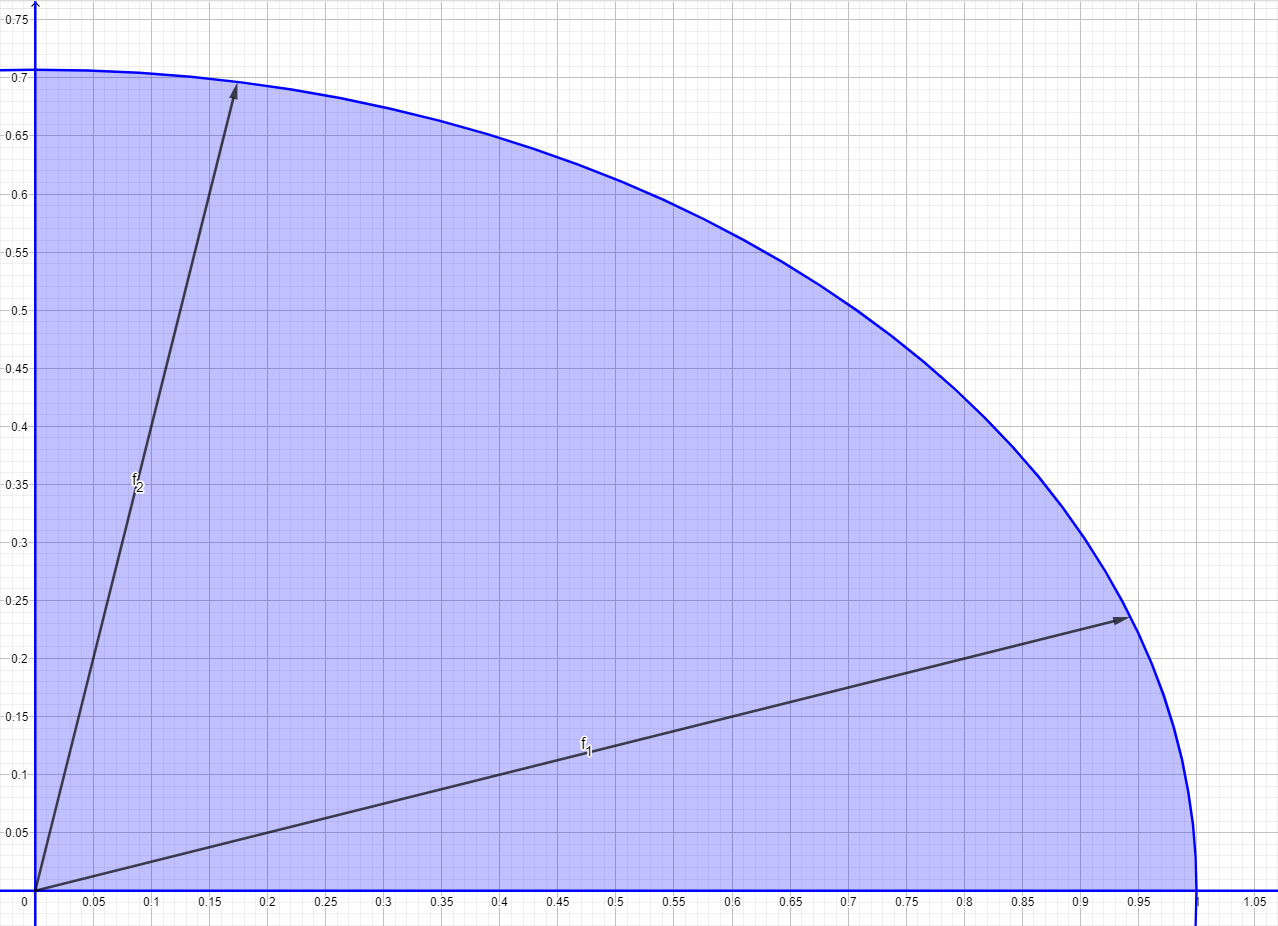
\includegraphics[width=\textwidth]{ideal_point_1.png}
    \end{figure}
    
    Далі знаходимо $a_i = \max_x f_i(x)$, $i = 1, 2$. Для цього спершу знаходимо $\tilde x_i = \arg \max f_i$. \\
    
    З графічних міркувань, $\tilde x_1$ -- точка дотику опорної прямої що перпендикулярна вектору $f_1$ (див. мал. вище) до допустимої області, тобто точка $\tilde x_1 = \left( \frac{8}{\sqrt{65}}, \frac{1}{\sqrt{2 \cdot 65}} \right)$, а відповідне значення \[ a_1 = f_1(\tilde x_1) = 4 \cdot \frac{8}{\sqrt{65}} + \frac{1}{\sqrt{2 \cdot 65}} = \frac{1 + 32 \sqrt{2}}{\sqrt{2 \cdot 65}}. \]
    
    Аналогічно знаходимо $\tilde x_2 = \left( \frac{1}{\sqrt{5}}, \frac{\sqrt{2}}{\sqrt{5}}\right)$, а відповідне значення \[ a_2 = f_2(\tilde x_2) = \frac{1}{\sqrt{5}} + 4 \cdot \frac{\sqrt{2}}{\sqrt{5}} = \frac{1 + 4 \sqrt{2}}{\sqrt{5}}. \]
    
    Далі записуємо \[ \rho_1(f(x), a) =  \left( \frac{1 + 32 \sqrt{2}}{\sqrt{2 \cdot 65}} - 4 x_1 - x_2 \right) + \left( \frac{1 + 4 \sqrt{2}}{\sqrt{5}} - x_1 - 4 x_2 \right) \to \min. \]
    
    Ця задача еквівалентна задачі $x_1 + x_2 \to \max$ за умови $x_1^2 + 2 x_2^2 = 1$. \\
    
    Записуємо функцію Лагранжа цієї задачі \[ L(x_1, x_2, \lambda) = x_1 + x_2 + \lambda (x_1^2 + 2 x_2^2 - 1) \to \max. \]
    
    Знаходимо необхідні умови екстремуму
    \begin{equation*}
        \left\{
            \begin{aligned}
                \frac{\partial L}{\partial x_1} &= 1 + 2 \lambda x_1 = 0, \\
                \frac{\partial L}{\partial x_2} &= 1 + 4 \lambda x_2 = 0, \\
                \frac{\partial L}{\partial \lambda} &= x_1^2 + 2 x_2^2 - 1 = 0.
            \end{aligned}
        \right.
    \end{equation*}
    
    З цієї системи маємо $x_1 = -\frac{1}{2\lambda}$, а $x_2 = - \frac{1}{4\lambda}$, тобто $x_1 = 2 x_2$. \\
    
    Враховуючи $x_1^2 + 2 x_2^2 = 1$, остаточно знаходимо $x^\star = \left( \frac{2}{\sqrt{6}}, \frac{1}{\sqrt{6}} \right)$. \\
    
    У свою чергу $f(x^\star) = \left( \frac{6}{\sqrt{6}}, \frac{9}{\sqrt{6}} \right)$.
\end{solution}

\newpage

% \begin{problem*}[класна]
%     Розв'язати задачу багато-критеріальної оптимізації $3 x_1 + x_2 \to \max$, $x_1 + 2 x_2 \to \max$ з допустимою областю що визначається нерівностями $0 \le x_1, x_2 \le 4$, $x_1 + x_2 \le 5$ методом ідеальної точки з $s = 2$.
% \end{problem*}

% \begin{solution}
    
% \end{solution}

\begin{problem}
    Розв'язати задачу двох-критеріальної оптимізації \[ f_1 = 2 x_1 + x_2 \to \max, \quad f_2 = x_1 + 3 x_2 \to \max \] з допустимою областю що визначається нерівностями \[ x_1 + x_2 \le 4, \quad x_1 + 2 x_2 \le 6, \quad x_{1, 2} \ge 0 \] методом ідеальної точки з $s = 2$.
\end{problem}

\begin{solution}
    Перш за все зобразимо допустиму область:
    \begin{figure}[H]
        \centering
        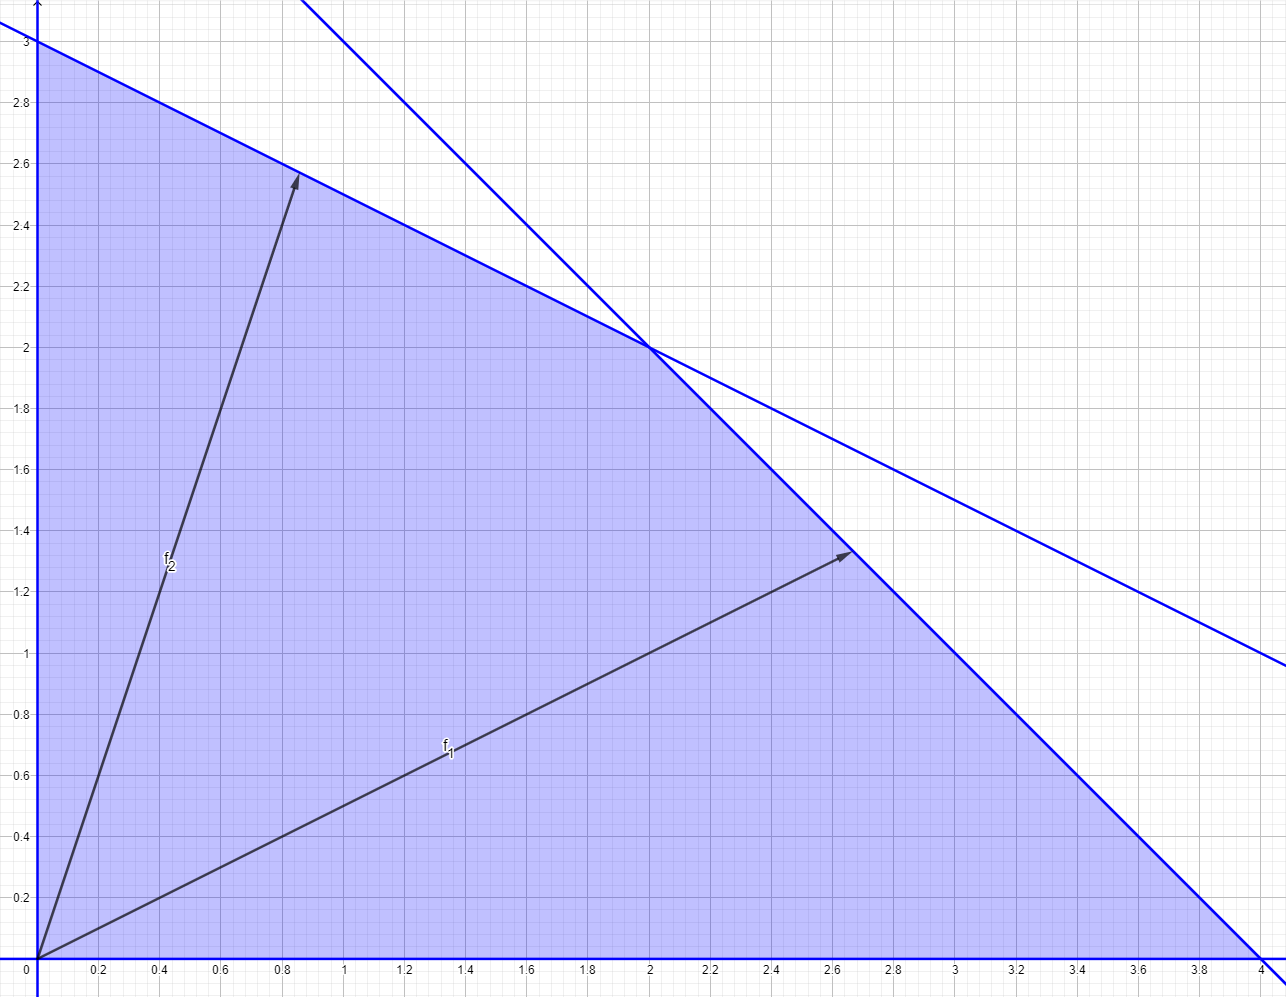
\includegraphics[width=\textwidth]{ideal_point_2.png}
    \end{figure}
    
    Далі знаходимо $a_i = \max_x f_i(x)$, $i = 1, 2$. Для цього спершу знаходимо $\tilde x_i = \arg \max f_i$. \\
    
    З графічних міркувань, $\tilde x_1$ --- точка дотику опорної прямої що перпендикулярна вектору $f_1$ (див. мал. вище) до допустимої області, тобто точка $\tilde x_1 = \left( 4, 0 \right)$, а відповідне значення \[ a_1 = f_1(\tilde x_1) = 2 \cdot 4 + 0 = 8. \]
    
    Аналогічно знаходимо $\tilde x_2 = \left( 0, 3 \right)$, а відповідне значення \[ a_2 = f_2(\tilde x_2) = 0 + 3 \cdot 3 = 9. \]
    
    Далі записуємо \[ \rho_2(f(x), a) = \left( 8 - 2 x_1 - x_2 \right)^2 + \left( 9 - x_1 - 3 x_2 \right)^2 \to \min. \]
    
    Записуємо функцію Лагранжа цієї задачі 
    \begin{multline*} 
        L(x_1, x_2, \lambda_1, \lambda_2) = \left( 8 - 2 x_1 - x_2 \right)^2 + \left( 9 - x_1 - 3 x_2 \right)^2 + \\ 
        + \lambda_1 \cdot (4 - x_1 - x_2) + \lambda_2 \cdot (6 - x_1 - 2 x_2) \to \min.
    \end{multline*}
    
    Знаходимо необхідні умови екстремуму
    \begin{equation*}
        \left\{
            \begin{aligned}
                \frac{\partial L}{\partial x_1} &= - 4 \cdot (8 - 2 x_1 - x_2) - 2 \cdot (9 - x_1 - 3 x_2) - \lambda_1 - \lambda_2 = 0, \\
                \frac{\partial L}{\partial x_2} &= - 2 \cdot (8 - 2 x_1 - x_2) - 6 \cdot (9 - x_1 - 3 x_2) - \lambda_1 - 2 \lambda_2 = 0, \\
                \frac{\partial L}{\partial \lambda_1} &= 4 - x_1 - x_2 = 0, \\
                \frac{\partial L}{\partial \lambda_2} &= 6 - x_1 - 2 x_2 = 0.
            \end{aligned}
        \right.
    \end{equation*}
    
    З цієї системи маємо $x^\star = \left( 2, 2 \right)$. \\
    
    У свою чергу $f(x^\star) = \left( 6, 8 \right)$.
\end{solution}

\newpage

% \begin{problem*}[класна]
%     Розв'язати задачу багато-критеріальної оптимізації $3 x_1 + x_2 \to \max$, $x_1 + 2 x_2 \to \max$ з допустимою областю що визначається нерівностями $0 \le x_1, x_2 \le 4$, $x_1 + x_2 \le 5$ методом ідеальної точки з $s = \infty$.
% \end{problem*}

% \begin{solution}
    
% \end{solution}

\begin{problem}
    Розв'язати задачу двох-критеріальної оптимізації \[ f_1 = x_1 \to \max, \quad f_2 = x_2 \to \max \] з допустимою областю що визначається нерівностями \[ 2 x_1 + x_2 \le 10, \quad x_1 + 3 x_2 \le 12, \quad x_1 + x_2 \le 6, \quad x_{1, 2} \ge 0 \] методом ідеальної точки з $s = \infty$.
\end{problem}

\begin{solution}
    Перш за все зобразимо допустиму область:
    \begin{figure}[H]
        \centering
        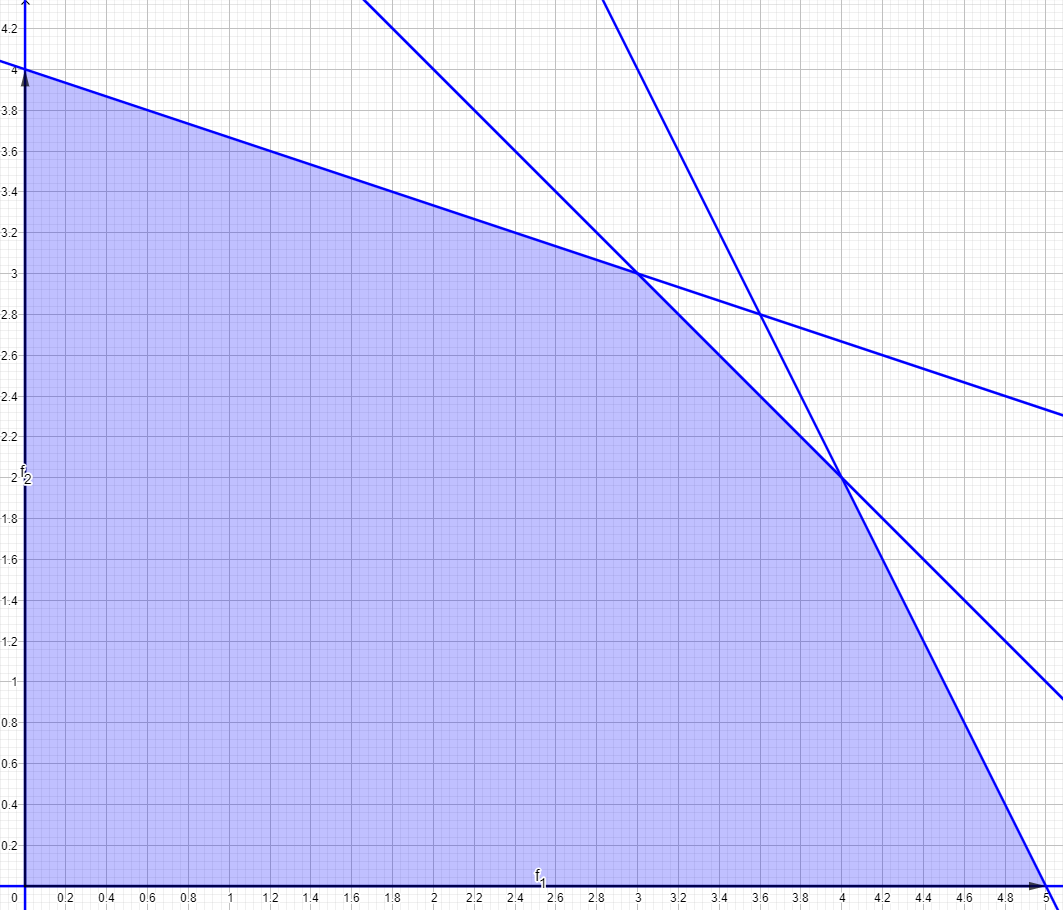
\includegraphics[width=\textwidth]{ideal_point_3.png}
    \end{figure}
    
    Далі знаходимо $a_i = \max_x f_i(x)$, $i = 1, 2$. Для цього спершу знаходимо $\tilde x_i = \arg \max f_i$. \\
    
    З графічних міркувань, $\tilde x_1$ -- точка дотику опорної прямої що перпендикулярна вектору $f_1$ (див. мал. вище) до допустимої області, тобто точка $\tilde x_1 = \left( 5, 0 \right)$, а відповідне значення \[ a_1 = f_1(\tilde x_1) = 5. \]
    
    Аналогічно знаходимо $\tilde x_2 = \left( 0, 4 \right)$, а відповідне значення \[ a_2 = f_2(\tilde x_2) = 4. \]
    
    Далі записуємо \[ \rho_2(f(x), a) = \max\{ 5 - x_1, 4 - x_2\} \to \min. \]
    
    З логічних (які, щоправда, не справджуються для деяких неопуклих задача) міркувань, цей мінімум досягається на межі допустимої області де $5 - x_1 = 4 - x_2$. \\
    
    Враховуючи нерівності що обмежують допустиму область маємо $x^\star = \left( 2.5, 3.5 \right)$. \\
    
    У свою чергу $f(x^\star) = \left( 2.5, 3.5 \right)$.
\end{solution}

\newpage
    
\section*{11 березня 2019 р.}

\setcounter{problem}{0}

\begin{problem}
    Розв'язати задачу багато-критеріальної оптимізації \[ f_1 = - x_1 - x_2 \to \max, \quad f_2 = 2 x_1 + x_2 \to \max, \quad f_3 = x_1 + 3 x_2 \to \max \] з допустимою областю що визначається нерівностями \[ x_1 + x_2 \le 4, \quad x_1 + 2 x_2 \le 6, \quad x_{1, 2} \ge 0 \] методом послідовних поступок (величини поступок вибрати самостійно).
\end{problem}

\begin{solution}
    Перш за все зобразимо допустиму область $G_0$:
    \begin{figure}[H]
        \centering
        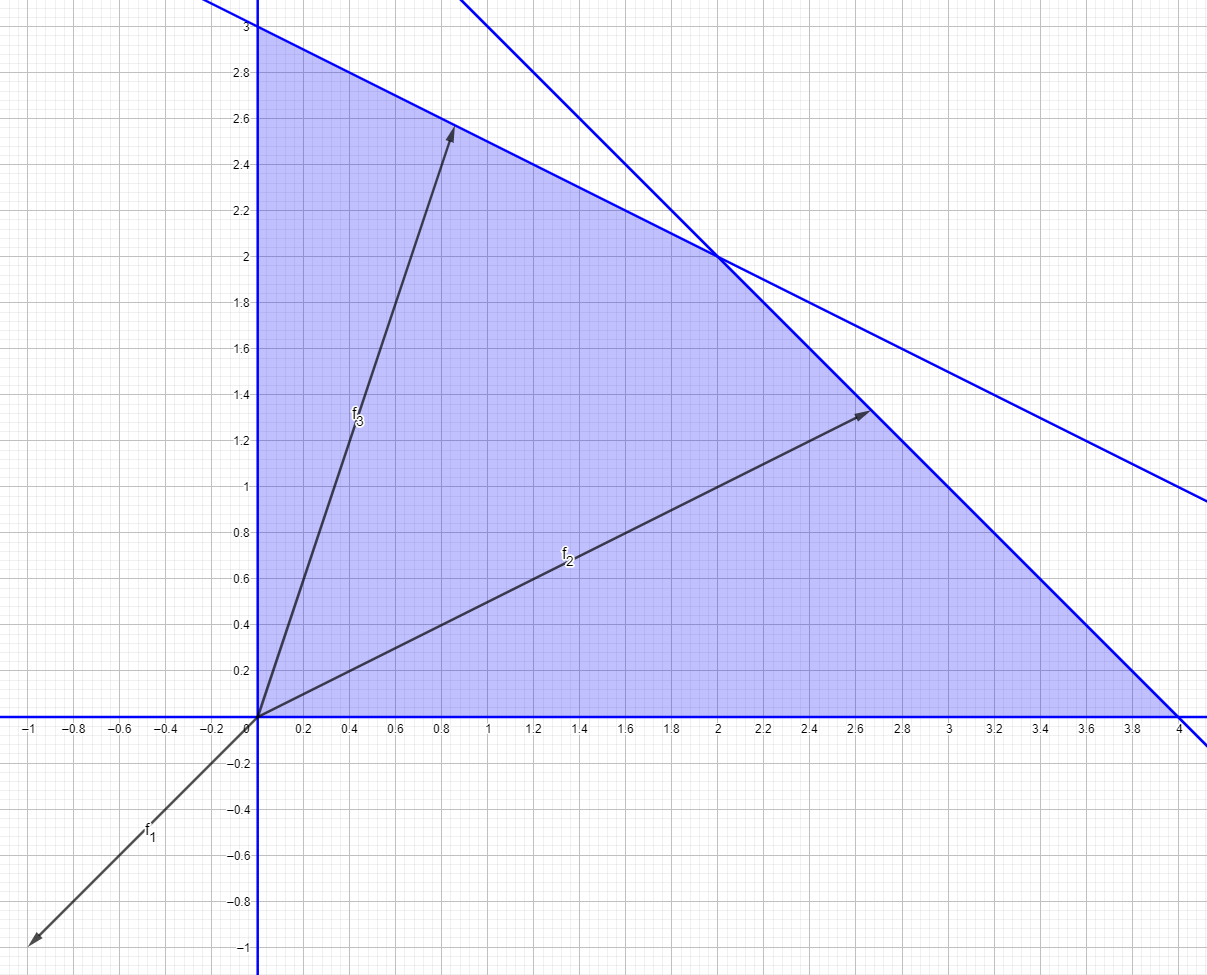
\includegraphics[width=\textwidth]{successive_concessions_1_1.png}
    \end{figure}

    З графічних міркувань знаходимо \[ \tilde x_1 = \arg \max f_1(x_1, x_2) = (0, 0), \quad f_1^\star = \max_{x \in G_0} f_1(x_1, x_2) = 0. \]
    
    Покладаючи величину поступки $\Delta f_1$ за першим критерієм рівною $2$ отримуємо, що до допустимої області додається умова \[ f_1(x_1, x_2) \ge f_1^\star - \Delta f_1 = -2, \] тому уточнена допустима область $G_1$ має вигляд:
    \begin{figure}[H]
        \centering
        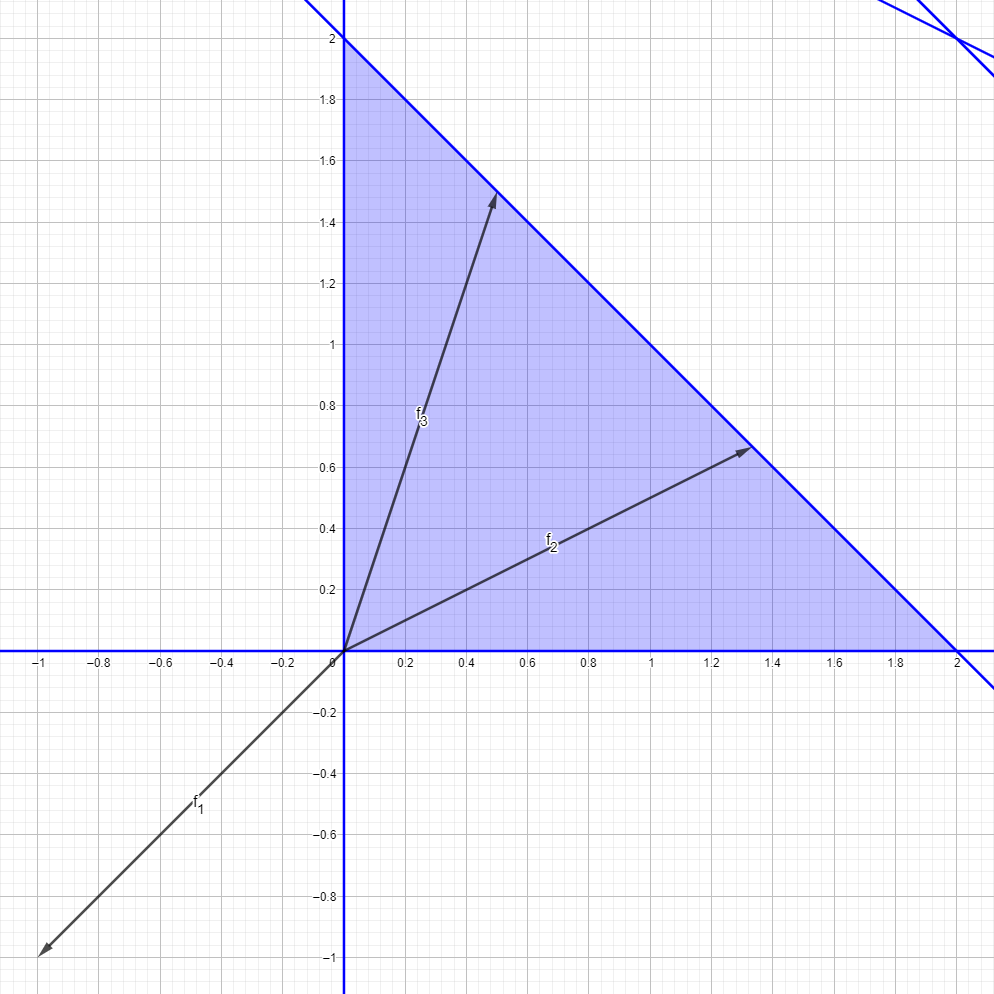
\includegraphics[width=\textwidth]{successive_concessions_1_2.png}
    \end{figure}

    З графічних міркувань знаходимо \[ \tilde x_2 = \arg \max f_2(x_1, x_2) = (2, 0), \quad f_2^\star = \max_{x \in G_1} f_2(x_1, x_2) = 4. \]
    
    Покладаючи величину поступки $\Delta f_2$ за другим критерієм рівною $2$ отримуємо, що до допустимої області додається умова \[ f_2(x_1, x_2) \ge f_2^\star - \Delta f_2 = 2, \] тому уточнена допустима область $G_2$ має вигляд:
    \begin{figure}[H]
        \centering
        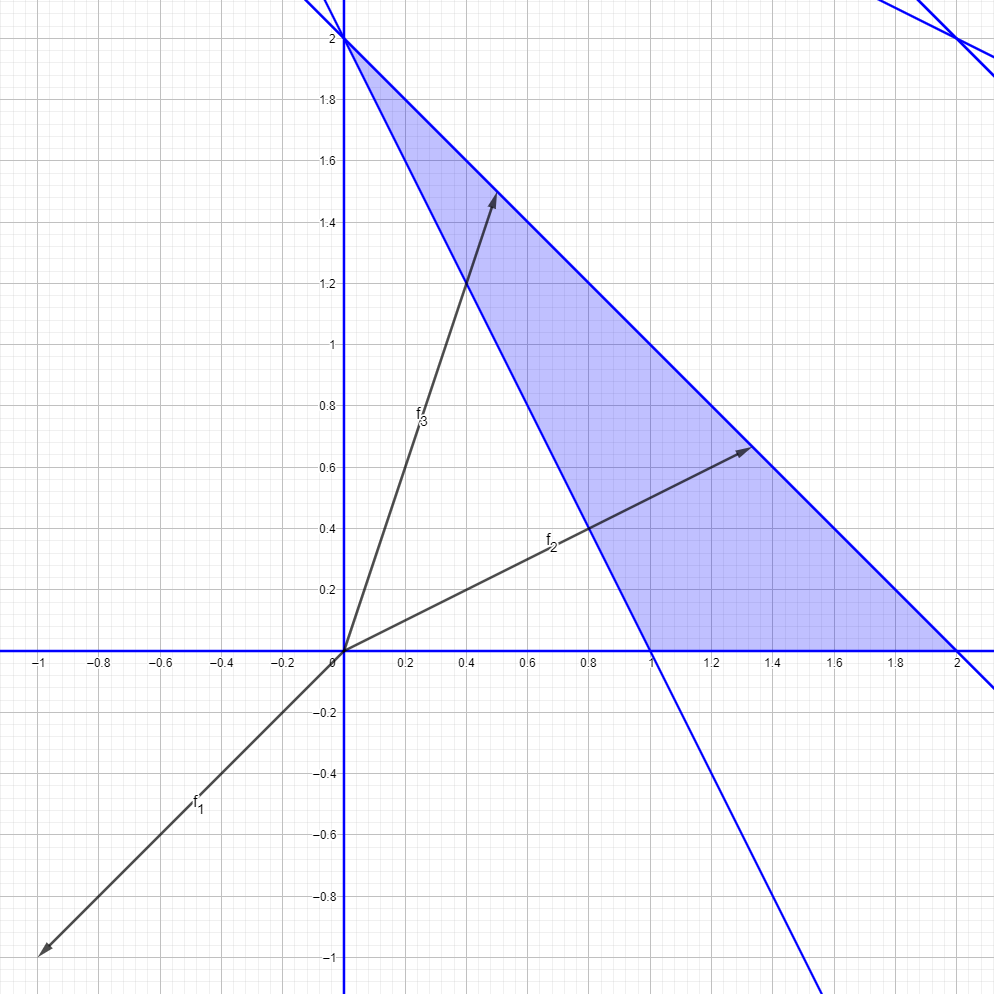
\includegraphics[width=\textwidth]{successive_concessions_1_3.png}
    \end{figure}

    З графічних міркувань знаходимо \[ \tilde x_3 = \arg \max f_3(x_1, x_2) = (0, 2), \quad f_3^\star = \max_{x \in G_2} f_3(x_1, x_2) = 6. \]
    
    Оскільки це останній критерій, то ми не робимо поступок, а просто кажемо, що знайдена точка $\tilde x_3$ є розв'язком $x^\star$. \medskip
    
    Наостанок зауважимо, що $f(x^\star) = (-2, 2, 6)$.
\end{solution}

\newpage

\begin{problem}
    Розв'язати задачу багато-критеріальної оптимізації \[ f_1 = - x_1 - 2 x_2 \to \max, \quad f_2 = 2 x_1 + x_2 \to \max, \quad f_3 = x_1 + 3 x_2 \to \max \] з допустимою областю що визначається нерівностями \[ x_1 + x_2 \le 4, \quad 2 x_1 + x_2 \le 6, \quad x_{1, 2} \ge 0 \] методом послідовних поступок (величини поступок вибрати самостійно).
\end{problem}

\begin{solution}
    Перш за все зобразимо допустиму область $G_0$:
    \begin{figure}[H]
        \centering
        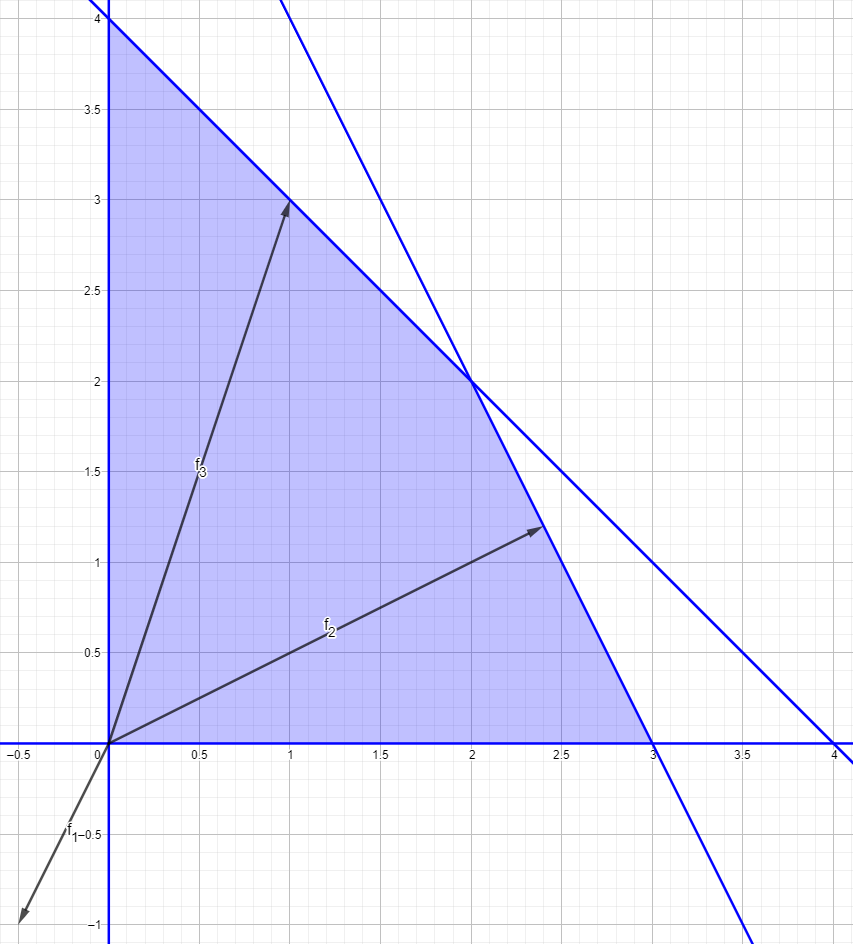
\includegraphics[width=\textwidth]{successive_concessions_2_1.png}
    \end{figure}

    З графічних міркувань знаходимо \[ \tilde x_1 = \arg \max f_1(x_1, x_2) = (0, 0), \quad f_1^\star = \max_{x \in G_0} f_1(x_1, x_2) = 0. \]
    
    Покладаючи величину поступки $\Delta f_1$ за першим критерієм рівною $4$ отримуємо, що до допустимої області додається умова \[ f_1(x_1, x_2) \ge f_1^\star - \Delta f_1 = -4, \] тому уточнена допустима область $G_1$ має вигляд:
    \begin{figure}[H]
        \centering
        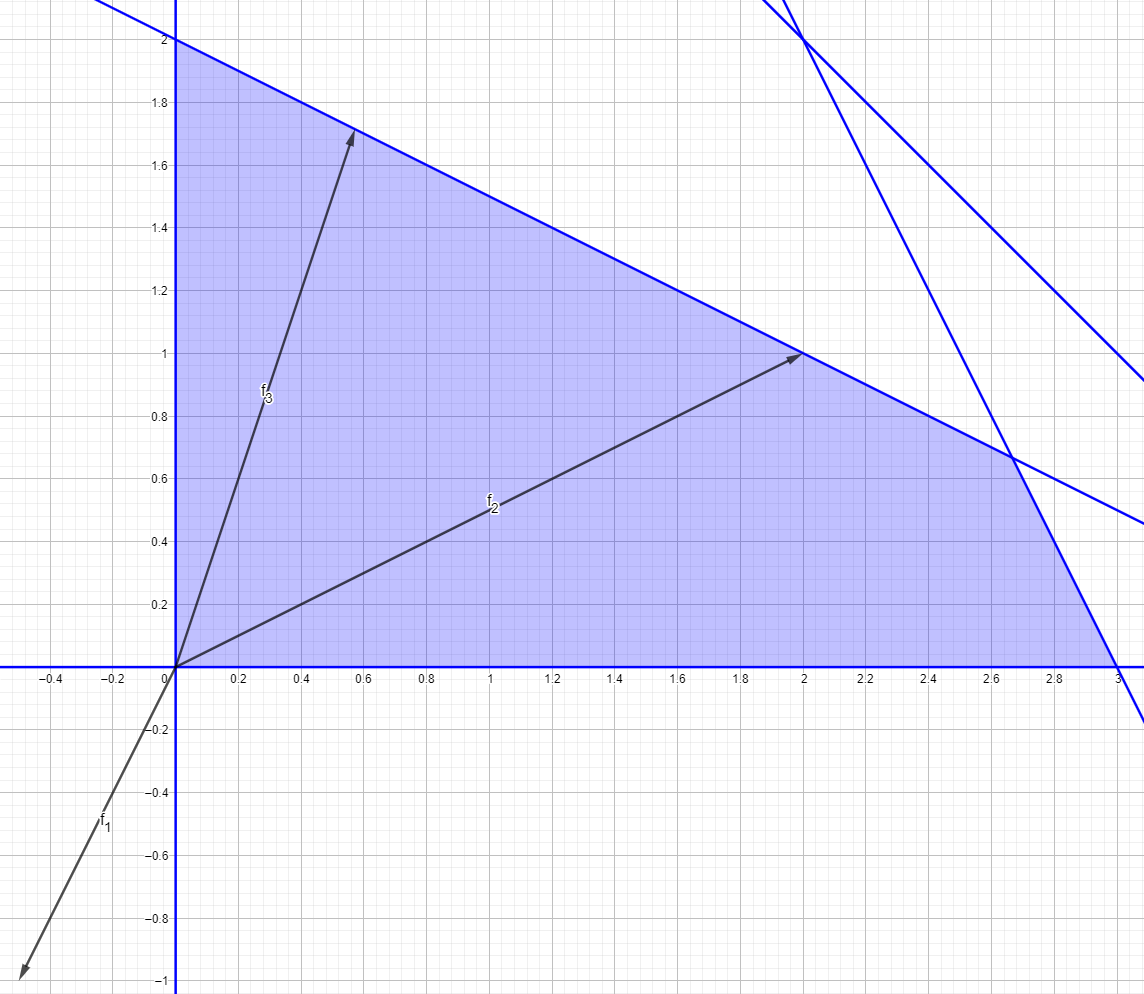
\includegraphics[width=\textwidth]{successive_concessions_2_2.png}
    \end{figure}

    З графічних міркувань знаходимо \[ \tilde x_2 = \arg \max f_2(x_1, x_2) = (3 - t, 2 t), \ t \in \left[0, \frac13\right], \quad f_2^\star = \max_{x \in G_1} f_2(x_1, x_2) = 6. \]

    Покладаючи величину поступки $\Delta f_2$ за другим критерієм рівною $3$ отримуємо, що до допустимої області додається умова \[ f_2(x_1, x_2) \ge f_2^\star - \Delta f_2 = 3, \] тому уточнена допустима область $G_2$ має вигляд:
    \begin{figure}[H]
        \centering
        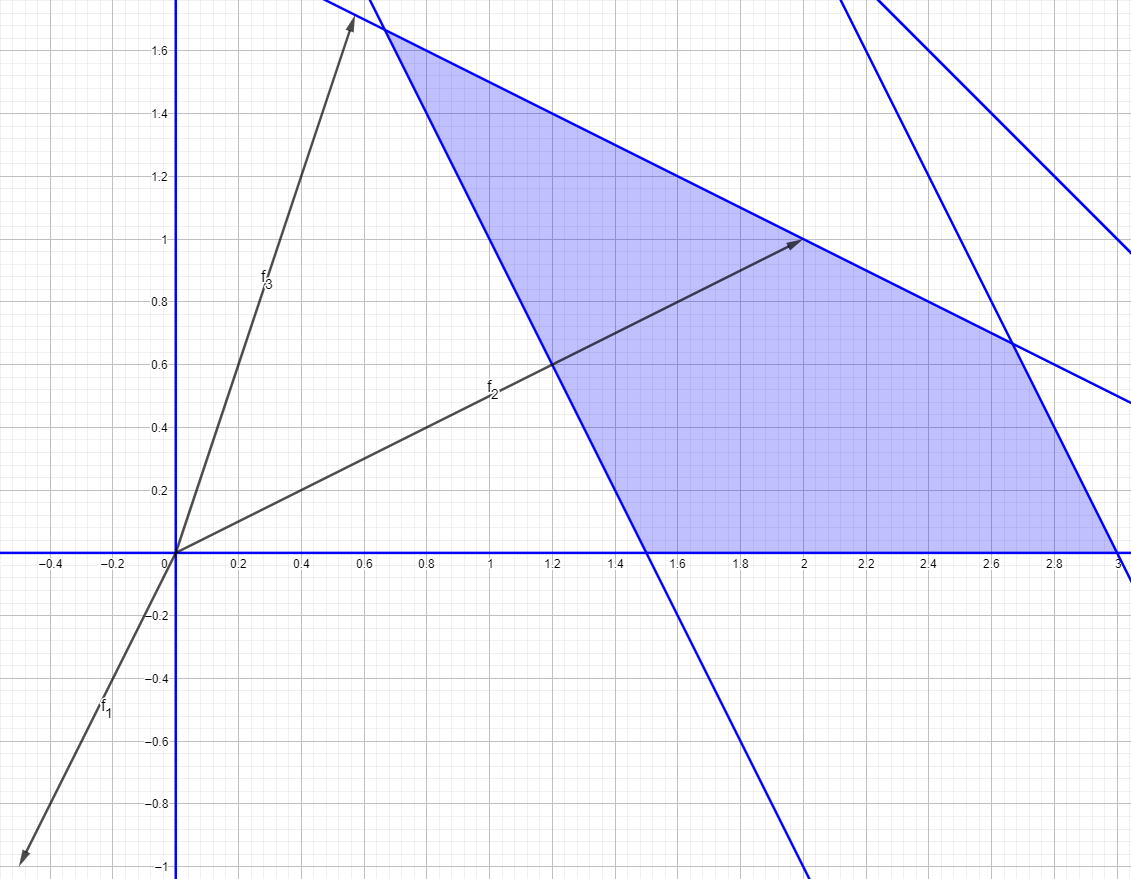
\includegraphics[width=\textwidth]{successive_concessions_2_3.png}
    \end{figure}

    З графічних міркувань знаходимо \[ \tilde x_3 = \arg \max f_3(x_1, x_2) = \left(\frac23, 1\ \frac23\right), \quad f_3^\star = \max_{x \in G_2} f_3(x_1, x_2) = 5\ \frac23. \]
    
    Оскільки це останній критерій, то ми не робимо поступок, а просто кажемо, що знайдена точка $\tilde x_3$ є розв'язком $x^\star$. \medskip
    
    Наостанок зауважимо, що \[ f(x^\star) = \left(-4, 3, 5\ \frac23\right).\]
\end{solution}

\end{document}